\section{Head Mounted Display}
\label{sec:hmd}

\begin{figure}[!b]
\centering
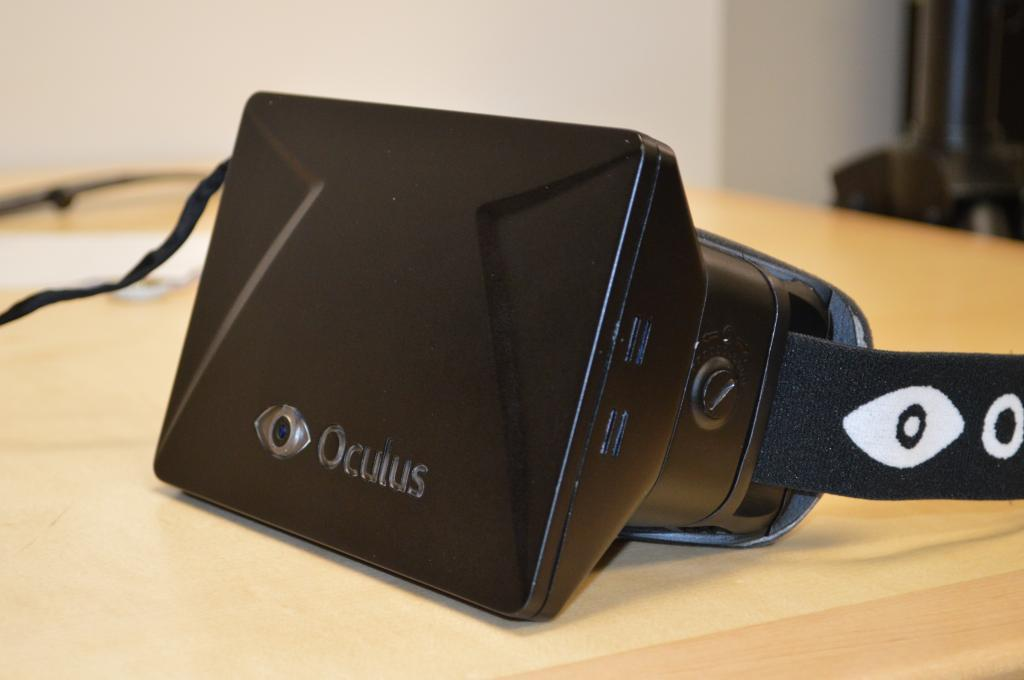
\includegraphics[width=0.5\textwidth]{oculus.jpg}
\caption{Oculus Rift Development Kit 1. 
\cite{website:pcworld}}
\label{fig:oculus}
\end{figure}

\begin{figure}[]
\centering
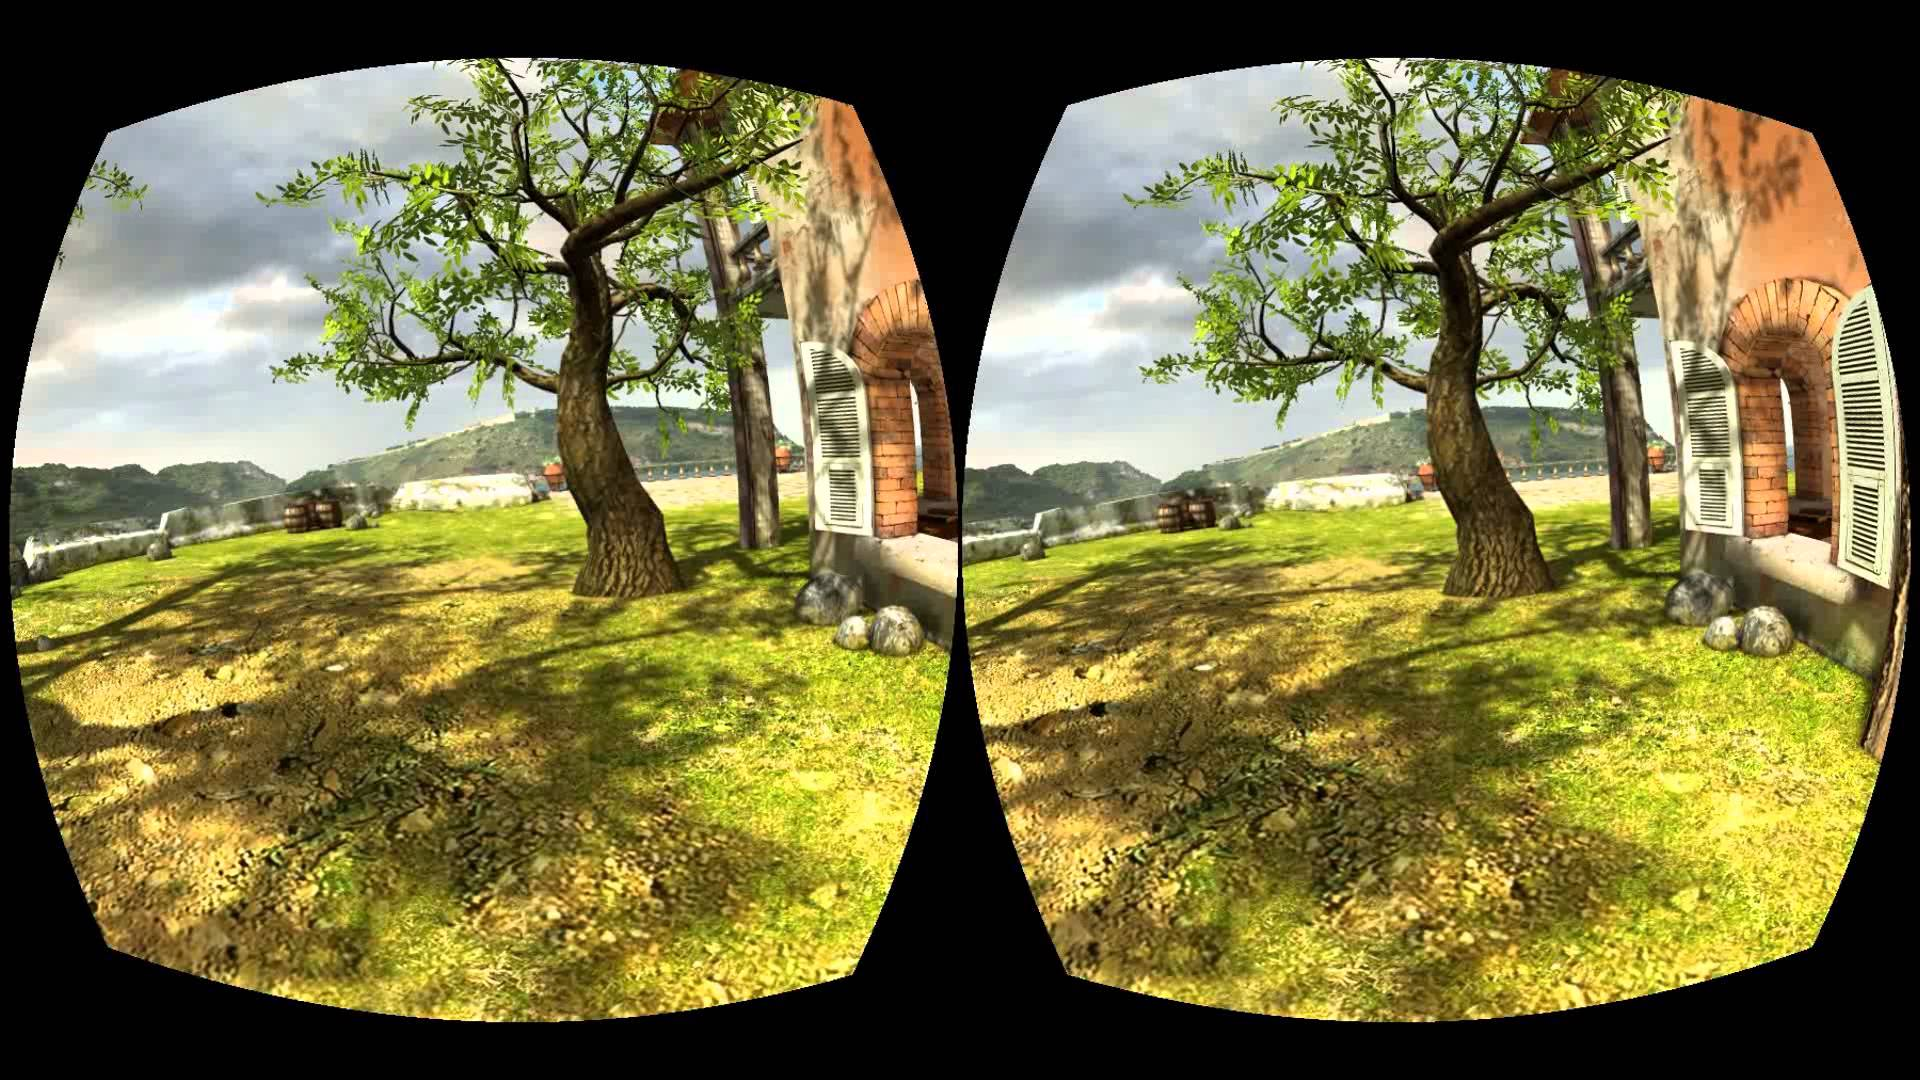
\includegraphics[width=0.5\textwidth]{stereoscopic.jpg}
\caption{A stereoscopic split screen view also rendered with barrel distortion.
Frames displayed on the Oculus screen appear normal.}
\label{fig:stereo}
\end{figure}

Since the Oculus Rift seen in Fig. \ref{fig:oculus} is the current state of the
art in HMD VR technology, it is a natural choice as the cornerstone for
graphical immersion in our system. The most simple applications one can develop
for the Oculus are created using basic OpenGL. The only caveat being that a
separate framebuffer must be bound to the context for off-screen rendering. The
framebuffer must have a texture bound to at as well which will be written to at
the last stage of the conventional pipeline. Parameters for constructing the
texture are provided directly from the Oculus SDK programatically.  The Oculus
SDK will then take the data placed in the texture and perform the
post-processing for stereoscopic 3D rendering and distortion processing. The
Oculus Rift requires a scene to be rendered in split-screen stereo. The left
eye sees the left half of the screen and the right eye sees the right half.
Human eye pupils are approximately 65 mm apart.  This interpupillary distance
(IPD) must be taken into consideration for configuring the in-application
camera.  Therefore, each scene is rendered twice, once for the virtual camera
on the left, and once for the virtual camera on the right. Both of which are
subject to a translation with respect to one another causing the stereoscopic
effect. The lenses in the Oculus provide a large degree of magnification in
order to provide a wide field of view so as to enhance immersion. However, as a
result the image succumbs to a great deal of pincushion distortion. To rectify
this distortion, the software must apply an equal and opposite amount of barrel
distortion. The final image rendered to the Oculus's display can be seen in
Fig. \ref{fig:stereo}. For the remainder of this paper, when discussing the
camera view, this refers to the single camera model provided to the Oculus SDK
before the post processing occurs. 

Graphics is known as the inverse problem to computer vision. Where computer
vision seeks to extract information about an environment from an image,
graphics seeks to extract information to construct an image from an
environment. What gives computer graphics the illusion of position and depth is
a mathematical process of constructing a series of transformations taking
arbitrary points from one frame of reference to another to infer position and
ultimately a projective transform to infer depth. The location of all 
the particles in an object can be defined with respect to some inertial frame
of reference. If one observes the object from some alternative location and
orientation with respect to the same intertial frame, one can construct a 
transformation to take points from the inertial frame to the view frame. This
is already well understood by many who have experience with 3D graphics

% Fix the orientation of the axis to reflect graphical frame
% \begin{figure}[b!]
% \centering
% 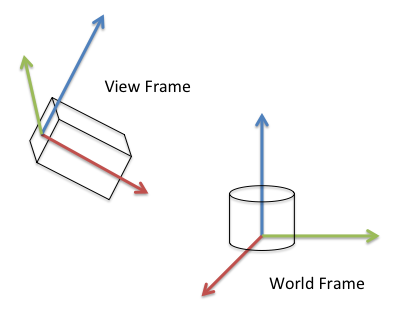
\includegraphics[width=0.5\textwidth]{world_view.png}
% \caption{Two frames of reference, the view and the world. The orienation and
% position of the view frame corresponds to the camera view.}
% \label{fig:worldview}
% \end{figure}

